\documentclass[11pt,a4paper]{report}
\usepackage[T1]{fontenc}
\usepackage[utf8]{inputenc}
\usepackage[english]{babel}
\usepackage{textcomp} % Euro symbols etc
\usepackage{graphicx} % support graphics
\usepackage{hyperref} % links in the document
\usepackage{float} % position of figures
\usepackage{paralist} % inline lists
\usepackage{verbatim} % multi-line comments
\usepackage{listings} % Syntax colored code
\usepackage{booktabs} % Professional tables
\usepackage{tabularx} % Simple column stretching
\usepackage{multirow} % Row spanning
\usepackage{wrapfig} % Wrap text around figures
\usepackage{amsmath} % Advanced maths
\usepackage[normalsize, bf]{caption} % Hide some tables from list of tables
\usepackage{array}
\usepackage{color}
\usepackage[Glenn]{fncychap}
\usepackage{fixltx2e}

\setcounter{tocdepth}{0} % Depth of table of contents

% Configure links in pdfs
\hypersetup{
    bookmarksopen=false, % Hide bookmarks menu
    colorlinks=true, % Don't wrap links in colored boxes
%    pdfborder={0 0 0} % Remove ugly boxes
}


%============
% Top matter
%============
\title{Group project}
\author{Even Wiik Thomassen, Terje Snarby, Weilin Wang}
\date{\today}

\begin{document}


%============
% Title page
%============
\begin{titlepage}
\begin{center}
% Upper part

\includegraphics[width=0.45\textwidth]{./img/NTNU-logo.png}\\[5cm]
\textsc{\large Department of Computer and Information Science}\\[0.2cm]
\textsc{\Large TDT4215 --- Web-Intelligence}\\[0.5cm]

% Title
\rule{\linewidth}{0.2mm} \\[0.4cm]
{ \LARGE \bfseries Project Report --- Group One}\\[0.2cm]
\rule{\linewidth}{0.2mm} \\[1.5cm]

% Author etc
\begin{minipage}{0.4\textwidth}
\begin{flushleft} \large
\emph{Authors:}\\
Even Wiik \textsc{Thomassen}\\
Terje \textsc{Snarby}\\
Weilin \textsc{Wang}
\end{flushleft}
\end{minipage}

% Bottom of the page
\vfill
{\large Word count: 4408}\\[0.2cm]
{\large \today}
\end{center}
\end{titlepage}


%==========
% Abstract
%==========
\begin{abstract}
Classifying treatment to patients can be complicated and error-prone. It could be beneficial to provide a system to health professionals that can automatically classify patient notes. We have created such a system with the help of vector space model based on TF-IDF and probabilistic model based on BM25F. This paper describes and evaluates such a system.
\end{abstract}


%===================
% Table of Contents
%===================
\pagenumbering{roman}
\clearpage
\phantomsection
\addcontentsline{toc}{chapter}{Contents}
\tableofcontents


%=================
% List of Figures
%=================
%\clearpage
%\phantomsection
%\addcontentsline{toc}{chapter}{List of figures}
%\listoffigures


%================
% List of Tables
%================
\setcounter{tocdepth}{1} % Depth of table of contents
\clearpage
\phantomsection
\addcontentsline{toc}{chapter}{List of tables}
\listoftables


%==========
% Chapters
%==========
\clearpage
\pagenumbering{arabic}
%---------------------
\chapter{Introduction}
%---------------------
This paper documents the mandatory group assignment in TDT4215 Web-intelligence
at Norwegian University of Science and Technology (NTNU).
TODO: describe the overall project goals

The paper is structured as follows:
\hyperref[cha:architecture]{Chapter \ref*{cha:architecture}} describes the
architecture of our system.
\hyperref[cha:method]{Chapter \ref*{cha:method}} explains methods used to
solve the project tasks, while \autoref{cha:result} presents results.
\hyperref[cha:discussion]{Chapter \ref*{cha:discussion}} provides a discussion
of the results, while \autoref{cha:conclusion} concludes the paper.
Stopwords, medical terms and patient cases are listed in the
\hyperref[appendix]{Appendix}.

%----------------------------
\chapter{System Architecture}
%----------------------------
\label{cha:architecture}
This chapter describes the architecture of our system. The system is build as
a decision support system for practitioners at a hospital. To prevent any
confusion, two roles are introduced.
\begin{description}
	\item[User] Practitioner that uses the system to search for relevant
				therapy chapters for a given patient case.
	\item[System administrator] Computer savvy personnel, in this case us, that
				manages the system. Doing the parsing of input files and
				building indices.
\end{description}

Our system consist of three logical parts: Python modules, input files, and
output files. There is also the external Python library Whoosh, used for
indexing and searching. In the following sections, each part will be explained
in detail. For an outline of the system, see \autoref{fig:systemarch}.

\begin{figure}[tbp]
	\noindent\makebox[\textwidth]{%
	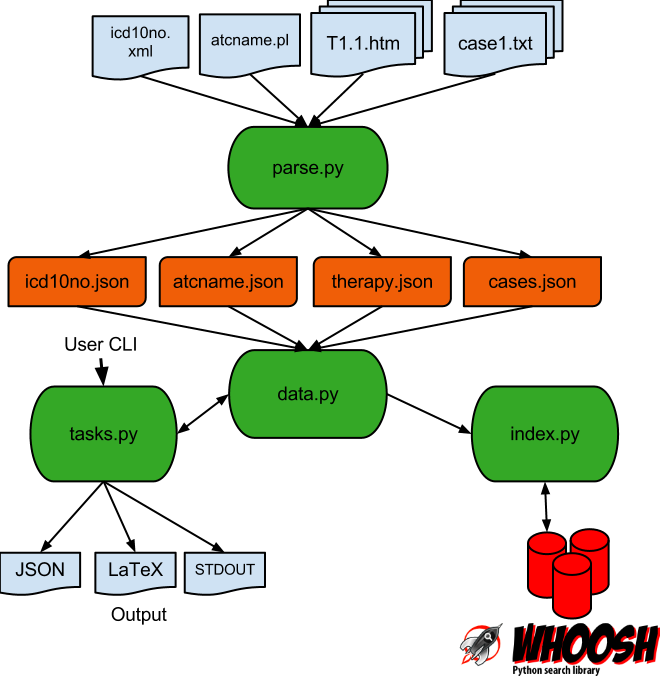
\includegraphics[width=1.1\textwidth]{./img/system_architecture2}}
	\caption{System overview\label{fig:systemarch}}
\end{figure}


\section{Whoosh}
%---------------
Whoosh\footnote{Whoosh: \url{http://pypi.python.org/pypi/Whoosh}} is a
search-engine library written in Python to support fast indexing and searching
of text collections. The library provides high performance, multifunctional
queries and support for scoring algorithms.

We use it to store, index and search on the four types of input data we must
handle: ICD-10 codes, ATC codes, therapy chapters, and patient cases. We only
use Whoosh search functionality for the first two tasks.


\section{Python modules}
%-----------------------
The system consists of four Python modules: parse.py, data.py, index.py, and tasks.py. Each module has its own features and tasks, and together they form the functional core of the system. The external Python library, Whoosh, provides index and search functionality to the core. In the following paragraphs each module is described in greater detail. For a full overview of the modules with their associated classes, attributes and methods, see the system's class diagram in \autoref{fig:classdiag}.

\begin{figure}[tbp]
	\noindent\makebox[\textwidth]{%
	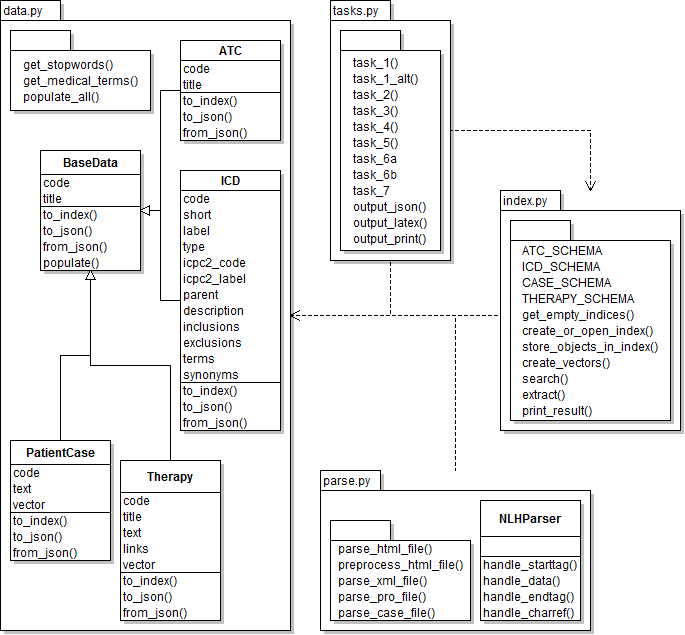
\includegraphics[width=1.1\textwidth]{./img/class_diagram}}
	\caption{Class diagram of the Python modules\label{fig:classdiag}}
\end{figure}

\paragraph{parse.py}
This module preprocess and converts input files to the more preferred JSON format, which gives better readability and reduces complexity for the following modules, which now only have to support one type of file. The module supports multiple file formats as input, for further information see the input files \autoref{sec:inputfiles}. The module is especially important for stripping out all the HTML tags from the therapy chapters. 

\paragraph{data.py}
The JSON files created by the parse module, are used as input to the data module. The data module holds representation of all the data the system needs. As a basis for holding the data we have the BaseData class, which is inherited by more specific classes for the different representations. As the system loads a JSON file, it determines which representation that should be used, ICD, ATC, PatientCase or Therapy. 

\paragraph{index.py}
Main module for building and managing the indices. After the data module has created the representation and holds the data, the index module can build indexes of it. This gives the system the ability to store text and to search for terms.

\paragraph{tasks.py}
This module contains the Command Line Interface (CLI), which makes the user able to interact with the system. The module contains methods to perform and solve the different tasks of the assignment, specified by the user. Output is generated by this module, either as STDOUT print or as a JSON- or LaTeX-file. Sample output can be seen in the appendices. 


\section{Input files}
%--------------------
\label{sec:inputfiles}
The system needs to support multiple file formats to be able to preprocess and parse the files given in the assignment. The ICD-10 file is a .xml file, the ATC file is a .pro file, the ``Norsk Legemiddel Håndbok'' is HTML and the cases are .txt files. So the parse module has support for files ending with: .xml, .pro, .htm and .txt. 


\section{Output files}
%---------------------
The result of the system is always presented in the command line. To be able to store the results and present them in this report, it was necessary and beneficial for us to make an output feature. The system is able to print the results to a JSON- or LaTeX-file. 
Storing results in JSON files are necessary to be able to use them for other tasks, such as task 6.



%---------------
\chapter{Method}
%---------------
This section describes TODO


\section{todo clever input data title}
%-------------------------------------
Describe how we plan to read in data files, parse them to generate objects
which we dump to json files. And why.

Describe how/why we also index things with Whoosh.

\subsection{ICD-10}
Describe what this is, how it is formatted, how we intend to preprocess and
parse it etc. And how we will store it in the Whoosh index, the schema.

\subsection{ATC}

\subsection{Legemiddelhandboka} % English?


\section{Tasks}
%--------------
Describe first methods which are used in several tasks, like Whoosh default
ranking method BM25F.
\url{http://packages.python.org/Whoosh/api/scoring.html#whoosh.scoring.BM27F}

Describe how and why we use stop words.

\subsection{Task 1 A}
Describe quick what the task is, what its inputs are.

\subsection{Task 1 B}

\subsection{Task 2 A}

\subsection{Task 2 B}

\subsection{Task 3}



%---------------
\chapter{Result}
%---------------
\label{cha:result}
This chapter presents results of the preprocessing and parsing of input files and the results from the assignment tasks. For task 1 and 2 we only present a subset of the results.

\section{Preprocessing and parsing}
%----------------------------------
The results of parsing the different input files can be seen in
\autoref{tab:objects}. Each code, chapter and case is stored in an object,
and saved to JSON files.
\begin{table}[htbp] \footnotesize \center
\caption{Parsed object counts\label{tab:objects}}
\begin{tabular}{l r}
    \toprule
    Type & Count \\
    \midrule
	ATC codes & 7945 \\
	ICD10 codes & 10521 \\
	Patient cases & 8 \\
	Therapy chapters & 917 \\
	\bottomrule
\end{tabular}
\end{table}

\autoref{tab:chapters} contains statistics showing the results of parsing
``Norsk legemiddelhåndbok'' HTML files --- therapy chapters. The statistics
lists the amount of chapters, in total and with text, for each of the
different chapter types --- from chapter to subsubsubsubchapter.
%Total amount of lines '\n': 3034
%Total amount of sentences '.': 24924
\begin{table}[htbp] \footnotesize \center
\caption{Therapy chapters statistics\label{tab:chapters}}
\begin{tabular}{l r r}
    \toprule
    Chapter type & Count & With text \\
    \midrule
	Chapter & 24 & 24 \\
	Subchapter & 153 & 104 \\
	Subsubchapter & 384 & 336 \\
	Subsubsubchapter & 329 & 326 \\
	Subsubsubsubchapter & 27 & 27 \\
    \midrule
	Total & 917 & 817 \\
	\bottomrule
\end{tabular}
\end{table}

Parsing of patient cases are summarized in \autoref{tab:cases}. Stopwords
refers to stopwords in the case text which have been removed, terms is the
number of unique terms (words) in the text.
\begin{table}[htbp] \footnotesize \center
\caption{Patient cases statistics\label{tab:cases}}
\begin{tabular}{c r r r r}
    \toprule
	Case \# & Lines & Stopwords & Terms & Medical terms \\
    \midrule
	1 & 13 & 1 & 55 & 10 \\
	2 & 22 & 1 & 169 & 24 \\
	3 & 17 & 0 & 125 & 30 \\
	4 & 6 & 1 & 49 & 4 \\
	5 & 11 & 2 & 63 & 14 \\
	6 & 7 & 0 & 41 & 9 \\
	7 & 20 & 2 & 123 & 29 \\
	8 & 12 & 0 & 90 & 19 \\
    \midrule
	Total & 108 & 7 & 715 & 125 \\
	\bottomrule
\end{tabular}
\end{table}

We store input data and results in JSON format, so we can work with them
without having to parse or produce them first. To demonstrate the
effectiveness of this method we list and compare the time (in seconds) it
takes to parse input data and loading JSON files in \autoref{tab:times}.
\begin{table}[htbp] \footnotesize \center
\caption{Comparing effectivenes of JSON\label{tab:times}}
\begin{tabular}{l r r c}
    \toprule
    Type & Parse time & JSON load time & Speedup \\
    \midrule
	ATC codes & 0.209 & 0.101 & 52\% \\
	ICD10 codes & 9.496 & 0.549 & 94\% \\
	Patient cases & 0.008 & 0.001 & 88\% \\
	Therapy chapters & 11.326 & 0.177 & 98\% \\
	\bottomrule
\end{tabular}
\end{table}


\section{Task 1: Autocoding ICD-10}
%----------------------------------
A sentence can match zero to many ICD-10 codes, but only the most specific shall be claimed as a match and presented in the results. Whoosh gives us a ranked list of the codes, and from this ranking the most specific code is selected. If there is more than one ICD-10 code that scores high and the match scores of the top results are close, the top three results are presented. If there is no match, a . is printed in the result table. This also applies to the therapy chapters and ATC-classifications. 

Autocoding of ICD-10 codes against patient case 1, 4, 5, and 6 can be seen in
\autoref{tab:task1a}, which list relevant ICD-10 codes for each sentence.
\autoref{tab:task1b} list results for task 1 B (therapy chapter T1.1.1, T5.5,
T8.9.2, and T24.2.1.7). Results for both method A and method B, described in
\autoref{sec:task1}, are listed next to each other for easy comparison.
\begin{table}[htbp] \footnotesize \center
\caption{Task 1 A, patient case 1, 4, 5, and 6\label{tab:task1a}}
\begin{tabular}{c c l l}
    \toprule
    Clinical note & Sentence & Method A & Method B \\
    \midrule
	1 & 1 & E10-E14 & E12, E10-E14, E14 \\
	 & 2 & E10-E14, E23.2 & E14 \\
	 & 3 & Y61.3 & Y61.3, Y62.3, Y60.3 \\
	 & 4 & Q02, P92.3 & P92.3 \\
	 & 5 & Z97.2, Q26.3 & Z97.2 \\
	 & 6 & . & E10-E14 \\
	 & 7 & . & . \\
	 & 8 & . & . \\
	 & 9 & O36.6 & P03.5 \\
	 & 10 & . & L85.3 \\
	 & 11 & . & . \\
	 & 12 & Z01.3 & Z34 \\
	 & 13 & Z38.1, Z38.0, Z38.3 & Y87.2 \\
	\addlinespace
	4 & 1 & O96 & M08, O96, R06.2 \\
	 & 2 & O33 & Q38.4 \\
	 & 3 & P92.4 & Z58.6 \\
	 & 4 & R96.0, N88.1, H91.2 & H91.2, M23.2 \\
	 & 5 & I20 & I20.1, I20 \\
	 & 6 & O84.0 & O84.0 \\
	\addlinespace
	5 & 1 & O26.2, N88.1 & O26.2, N91.1, N91.4 \\
	 & 2 & R15, R19.5 & R19.5, R19.4 \\
	 & 3 & Y65.0 & C77.8 \\
	 & 4 & O46.9 & . \\
	 & 5 & D83 & D83 \\
	 & 6 & S63.1 & S60.0 \\
	 & 7 & I84.3 & H60.0 \\
	 & 8 & C86.6 & R85 \\
	 & 9 & Q56.4, Q56, F70 & Q56, D57.3, M93.9 \\
	 & 10 & D80.6 & D80.6 \\
	 & 11 & Y61.4, Y62.4, Y60.4 & Y61.4, Y62.4, Y60.4 \\
	\addlinespace
	6 & 1 & R98, R59 & R98, R59.9, R59.0 \\
	 & 2 & R76.2 & R76.2 \\
	 & 3 & . & B90.9 \\
	 & 4 & D83, U80.0 & U80 \\
	 & 5 & E59, E58, E60 & U80 \\
	 & 6 & Y84.4 & P24.3 \\
	 & 7 & G81.0, G82.3, G82.0 & G81.0, G82.3, G82.0 \\
	\bottomrule
\end{tabular}
\end{table}

\begin{table}[htbp] \footnotesize \center
\caption{Task 1 B, chapter T1.1.1, T5.5, T8.9.2, and T24.2.1.7\label{tab:task1b}}
\begin{tabular}{c c l l}
    \toprule
    Chapter & Sentence & Method A & Method B \\
    \midrule
	T1.1.1 & 1 & B01, B01.9, B01.8 & B01.9, B01, B01.8 \\
	 & 2 & Z20, Z20.8, Z20.9 & A88.0, Z20, Z20.0 \\
	 & 3 & B01, B01.9, B01.8 & B01.9, B02.9, B02.8 \\
	 & 4 & C21.2 & O69.8 \\
	 & 5 & Q90.2 & C92.5 \\
	 & 6 & N92.4 & Z00.2 \\
	 & 7 & R00-R99 & R00-R99 \\
	 & 8 & P36.2 & A41.0, B95.6, G11.9 \\
	 & 9 & G11.1 & B01.2†, G11.1, G11.9 \\
	 & 10 & B01 & B01, B01.9, B01.8 \\
	\addlinespace
	T5.5 & 1 & F68.0, Z53.8, Z41.9 & R19.6 \\
	 & 2 & U00-U49, Z31.5, Q95.4 & Z90.5, U00-U49, I25.2 \\
	 & 3 & F32.8 & F33, F32.8 \\
	 & 4 & F51.2 & R41.8, R41, E23 \\
	 & 5 & F41.0, F32.3, F32.2 & F32.2, F32.3, F33.2 \\
	 & 6 & F31.3 & F33.3, F33.2 \\
	 & 7 & F31.8 & R70.0, F52, I51 \\
	 & 8 & F31.4, F31.5 & F33.3 \\
	 & 9 & Z34.9, Q97.1, F32.8 & Z34.9, O84.0 \\
	 & 10 & Z29, Z29.9 & F33.3, F31.8, Z29 \\
	 & 11 & O15.9 & Y4N \\
	 & 12 & Z55.0 & R45.4, R19.6, R46.0 \\
	 & 13 & P91.4, F20.4 & F60-F69 \\
	\addlinespace
	T8.9.2 & 1 & O42.1, O42.0 & O02.9, O02.8, G45.9 \\
	 & 2 & O96, Z00.8, I63 & O96, I63.3 \\
	 & 3 & G45.9, J46 & A50.0 \\
	 & 4 & Z00, A52.2, I48 & Z00, Z92.2, Z03 \\
	 & 5 & B20-B24 & I67, I68.0 *, I67.8 \\
	\addlinespace
	T24.2.1.7 & 1 & Z56.6 & F43 \\
	 & 2 & K59.1, O34, O35 & I22 \\
	 & 3 & I20 & I20.0, I20.1, I22 \\
	 & 4 & P08.0, Y61.3, Y62.3 & Y61.3, Y62.3, Y60.3 \\
	 & 5 & O63, P92.5, L21.1 & O63, R68.1, U00-U99 \\
	 & 6 & J46, I20, I20.0 & I20.0, I44.1 \\
	 & 7 & O42.1, O42.0 & F51.2, R96.1, F20.6 \\
	 & 8 & O42.1, O42.0, Z39.0 & T80.1, T80.2, T80 \\
	 & 9 & T32.3 & Z53 \\
	\bottomrule
\end{tabular}
\end{table}


\section{Task 2: Autocoding ATC}
%-------------------------------
Autocoding of ATC codes against patient case 1, 2, 3, 7, and 8 can be seen in
\autoref{tab:task2a}, where each sentence in patient cases are listed with
relevant ATC codes. \autoref{tab:task2b} list relevant ATC codes for therapy
chapter T1.10, T2.2.5.1, T3.1, and T6.2.3.
\begin{table}[htbp] \footnotesize \center
\caption{Task 2 A, patient case 1, 2, 3, 7, and 8\label{tab:task2a}}
\begin{tabular}{c c l c l}
    \toprule
    Case & Sentence & ATC codes & Sentence & ATC codes \\
    \midrule
	1 & 1 & A10X & 8 & . \\
	 & 2 & A10X & 9 & A10AD \\
	 & 3 & A10AE & 10 & . \\
	 & 4 & . & 11 & . \\
	 & 5 & A10AB1 & 12 & . \\
	 & 6 & . & 13 & . \\
	 & 7 & . & & \\
	\addlinespace
	2 & 1 & . & 12 & . \\
	 & 2 & . & 13 & . \\
	 & 3 & . & 14 & A10AD1 \\
	 & 4 & . & 15 & . \\
	 & 5 & N1BB1 & 16 & . \\
	 & 6 & . & 17 & . \\
	 & 7 & D8AC2 & 18 & . \\
	 & 8 & . & 19 & . \\
	 & 9 & . & 20 & V3AN5, G3AA7, G3AA12 \\
	 & 10 & . & 21 & R3BB1, R3BA2, R3AC3 \\
	 & 11 & V4CX & 22 & A10AD1 \\
	\addlinespace
	3 & 1 & C1BA & 10 & . \\
	 & 2 & . & 11 & . \\
	 & 3 & . & 12 & J1CE1, D6AX2, D10AF3 \\
	 & 4 & J7BB1 & 13 & N5BA1 \\
	 & 5 & . & 14 & . \\
	 & 6 & A10AD1 & 15 & . \\
	 & 7 & . & 16 & . \\
	 & 8 & . & 17 & . \\
	 & 9 & . & & \\
	\addlinespace
	7 & 1 & . & 11 & N2 \\
	 & 2 & V9B & 12 & N2BE1, M1AE2, M1AE2 \\
	 & 3 & . & 13 & M1AE2, M1AE2 \\
	 & 4 & . & 14 & N2AA59, N2AA59 \\
	 & 5 & . & 15 & N2AB1 \\
	 & 6 & . & 16 & B5BB \\
	 & 7 & . & 17 & V10B \\
	 & 8 & . & 18 & N2AA1 \\
	 & 9 & . & 19 & N2AA1, N2AA1 \\
	 & 10 & . & 20 & N2A, Z9OP, Z9SA \\
	\addlinespace
	8 & 1 & C1BA & 7 & V4CB \\
	 & 2 & . & 8 & V4CB \\
	 & 3 & A7AA, D1AA, G1AA & 9 & . \\
	 & 4 & V4CB & 10 & A12AA12 \\
	 & 5 & . & 11 & R1AX \\
	 & 6 & J1CE2, J1CE1 & 12 & C2N \\
	\bottomrule
\end{tabular}
\end{table}

\begin{table}[htbp] \footnotesize \center
\caption{Task 2 B, chapter T1.10, T2.2.5.1, T3.1, and T6.2.3\label{tab:task2b}}
\begin{tabular}{c c l c l}
    \toprule
    Chapter & Sentence & ATC codes & Sentence & ATC codes \\
    \midrule
	T1.10 & 1 & C5A, D5A, A1AB & 6 & J1EE1, J1RA1 \\
	 & 2 & V7, V7A & 7 & C10AC, N5BA1, M4AB \\
	 & 3 & V9D, J1EB, A7EC1 & 8 & A5AB, D5BB, D10AF \\
	 & 4 & J7BC20, A7EC1, N4AC & 9 & V4CB, V4CD, V4CG \\
	 & 5 & B1AD12, B5A, C8D & 10 & J7BC20, A7EC1 \\
	\addlinespace
	T2.2.5.1 & 1 & M4AA, L3AB1, L3AB4 & 2 & A5AB, D5BB, D10AF \\
	\addlinespace
	T3.1 & 1 & C2LG51, A10X, V3AA & 23 & V3AH \\
	 & 2 & C10AC, M4AB, H2AB & 24 & H4AA1, Z0CA, A5AB \\
	 & 3 & B5D, B5BA3, B5CX1 & 25 & A5AB, D5BB, D10AF \\
	 & 4 & A10BX2, A10BX3, Z0ET & 26 & B5BA3, B5CX1, V4CA2 \\
	 & 5 & B5BB, G3, M5B & 27 & V9DX1 \\
	 & 6 & V6DB & 28 & A14A \\
	 & 7 & A10AD1 & 29 & B5BC2, D2AE1, B5BA3 \\
	 & 8 & A10BA2, Z9MF, A10BD2 & 30 & A10AE, B5BB3, B5BB \\
	 & 9 & A10AE & 31 & V7AD \\
	 & 10 & A10BD, J7BC20, A10AD1 & 32 & A10AB1, A10AD4 \\
	 & 11 & V3AH & 33 & . \\
	 & 12 & A7EC1, N4AC & 34 & V3AH \\
	 & 13 & B5BA3, B5CX1, V4CA2 & 35 & A10X, N4AC, N7 \\
	 & 14 & A10AE & 36 & C5BA, C5AX, C5BB \\
	 & 15 & A10BD3 & 37 & Z9AC \\
	 & 16 & A10AE4, A10AE5 & 38 & Z9ST, V9G \\
	 & 17 & A10AE & 39 & A5AX, M4AC, A7EC1 \\
	 & 18 & A10AC1, N4AC & 40 & Z9A2 \\
	 & 19 & C9AA5, A10AB, A10B & 41 & C10AC, M4AB, A10BA2 \\
	 & 20 & A10AC1, A10AB & 42 & . \\
	 & 21 & J4AK, S1KX, P1A & 43 & Z9AC \\
	 & 22 & V3AH, J4AK, M9AX & 44 & J4AK, V4CB, V4CD \\
	 & & & 45 & A1AB \\
	\addlinespace
	T6.2.3 & 1 & V3AA, N4AC & 4 & V9G, V4CB, V4CD \\
	 & 2 & S3, V4CJ, A7EC1 & 5 & V3AA, N3AX12, Z9BD \\
	 & 3 & N4AC & & \\
	\bottomrule
\end{tabular}
\end{table}


\section{Task 3: Ranking using vector models}
%--------------------------------------------
Ranked lists of relevant therapy chapters for each patient case can be found
in \autoref{tab:task3a} and \autoref{tab:task3b}.
\begin{table}[htbp] \footnotesize \center
\caption{Task 3 results (part 1)\label{tab:task3a}}
\begin{tabular}{c c c l}
    \toprule
    Case & Rank & Score & Relevant chapter \\
    \midrule
    1 & 1 & 0.08 & T3.1: Diabetes mellitus \\
     & 2 & 0.04 & T10.2.1: Bronkial astma \\
     & 3 & 0.04 & T14.5.1: Polycystisk ovarialt syndrom (PCOS) \\
     & 4 & 0.04 & T23.1.1.2: Faste og stress \\
     & 5 & 0.04 & T5.4.1: Schizofreni \\
     & 6 & 0.03 & T14.2.1: Forskyvning av normal menstruasjon \\
     & 7 & 0.03 & T10.2.1.1: Mild og moderat astma \\
     & 8 & 0.03 & T18.1.4: Kontroll og oppfølging \\
     & 9 & 0.03 & T16.13.1: Generalisert kløe \\
     & 10 & 0.03 & T9.1.5: Anafylaktoide reaksjoner \\
	\addlinespace
    2 & 1 & 0.08 & T10.2: Obstruktiv lungesykdom \\
     & 2 & 0.06 & T10.2.2: Kronisk obstruktiv lungesykdom (kols) \\
     & 3 & 0.05 & T8.4.1.2.2: Atrioventrikulær nodal reentrytakykardi \\
     & 4 & 0.05 & T10.2.1: Bronkial astma \\
     & 5 & 0.04 & T8.3.2.2: Hjerteinfarkt med ST-elevasjon \\
     & 6 & 0.04 & T3.1: Diabetes mellitus \\
     & 7 & 0.04 & T10.8: Sarkoidose \\
     & 8 & 0.04 & T15.3.7: Liten melkeproduksjon \\
     & 9 & 0.03 & T5.3.1.3: Alkohol abstinensreaksjoner \\
     & 10 & 0.03 & T6.2.2: Klasehodepine («Cluster headache») \\
	\addlinespace
    3 & 1 & 0.09 & T1.10: Akutt bakteriell meningitt \\
     & 2 & 0.05 & T3.1: Diabetes mellitus \\
     & 3 & 0.05 & T8.1: Hypertensjon \\
     & 4 & 0.05 & T1.11: Bakteriell endokarditt \\
     & 5 & 0.04 & T16.7.1: Skabb \\
     & 6 & 0.04 & T8.2.1: Malign hypertensjon \\
     & 7 & 0.04 & T19.1: Feber \\
     & 8 & 0.04 & T8.2.2: Hypertensjonsencefalopati \\
     & 9 & 0.04 & T8.3.2.2: Hjerteinfarkt med ST-elevasjon \\
     & 10 & 0.04 & T14.6.4: Akutt bekkeninfeksjon \\
	\addlinespace
    4 & 1 & 0.09 & T8.3: Koronarsykdom \\
     & 2 & 0.06 & T11.1.1.4.7: Emosjonell rhinitt \\
     & 3 & 0.05 & T8.2.4: Hypertensjonskrise og hjerteinfarkt eller ustabil angina \\
     & 4 & 0.05 & T4.6.3: Arteriell trombose \\
     & 5 & 0.04 & T8.3.1: Stabil koronarsykdom (stabil angina pectoris) \\
     & 6 & 0.04 & T8.4.1.2: Paroksystisk supraventrikulær takykardi \\
     & 7 & 0.04 & T10.2.2: Kronisk obstruktiv lungesykdom (kols) \\
     & 8 & 0.04 & T8.3.2.1: Ustabil angina/hjerteinfarkt uten ST-elevasjon \\
     & 9 & 0.04 & T24.2.1.7: Myokardscintigrafi \\
     & 10 & 0.03 & T15.3.7: Liten melkeproduksjon \\
	\bottomrule
\end{tabular}
\end{table}

\begin{table}[htbp] \footnotesize \center
\caption{Task 3 results (part 2)\label{tab:task3b}}
\begin{tabularx}{\textwidth}{c c c X}
    \toprule
    Case & Rank & Score & Relevant chapter \\
    \midrule
    5 & 1 & 0.06 & T12.10.1: Hemoroider \\
     & 2 & 0.06 & T12.9.3: Dyschezi (rektumobstipasjon) \\
     & 3 & 0.05 & T4.1: Anemier \\
     & 4 & 0.05 & T1.6.2.1: Clostridium difficile enterokolitt \\
     & 5 & 0.05 & T12.10.3: Fissura ani \\
     & 6 & 0.05 & T12.11: Familiær adenomatøs polypose \\
     & 7 & 0.05 & T5.5: Depresjoner \\
     & 8 & 0.04 & T15.1.5: Svangerskapsindusert hypertensjon \\
     & 9 & 0.04 & T4.1.3.2: Talassemi \\
     & 10 & 0.04 & T13.2.5: Nevrogene blæreforstyrrelser \\
	\addlinespace
    6 & 1 & 0.06 & T2.2.5.1: Cancer i nyreparenkym og binyre \\
     & 2 & 0.05 & T11.3.2.2: Kronisk tonsillitt \\
     & 3 & 0.04 & T11.3.1.2: Kronisk faryngitt \\
     & 4 & 0.04 & T1.7.7: Lymfogranuloma venereum \\
     & 5 & 0.04 & T11.4.4: Halitosis \\
     & 6 & 0.04 & T1.1.8: Skarlagensfeber \\
     & 7 & 0.03 & T11.3.2.1: Akutt tonsillitt \\
     & 8 & 0.03 & T1.6.1: Ikke-inflammatoriske, toksinpregete enteritter \\
     & 9 & 0.03 & T10.3.4: Pneumonier, bakterielle og med ukjent etiologi \\
     & 10 & 0.03 & T10.2.1.1: Mild og moderat astma \\
	\addlinespace
    7 & 1 & 0.08 & T6.2.3: Spenningshodepine (Tensjonshodepine) \\
     & 2 & 0.07 & T20.2.1: Akutte smerter \\
     & 3 & 0.06 & T21.1.1.2: Nevropatiske smerter \\
     & 4 & 0.06 & T20.2.3.1: Praktisk gjennomføring av smertebehandling hos pasienter med kort livsprognose \\
     & 5 & 0.06 & T22.4.1.1: Postoperativ grunnanalgesi \\
     & 6 & 0.06 & T20.1.2.2: Opioidanalgetika \\
     & 7 & 0.06 & T20.2.2.1: Praktisk gjennomføring av smertebehandling hos pasienter med antatt normal levetid \\
     & 8 & 0.06 & T21.1.1.1: Nociseptive smerter \\
     & 9 & 0.05 & T20.2.3.2: Bruk av sterkere opioider hos pasienter med kort livsprognose \\
     & 10 & 0.04 & T6.5.1: Multippel sklerose \\
	\addlinespace
    8 & 1 & 0.08 & T11.3.2.1: Akutt tonsillitt \\
     & 2 & 0.06 & T1.1.8: Skarlagensfeber \\
     & 3 & 0.04 & T1.7.5: Syfilis \\
     & 4 & 0.04 & T11.3.1.1: Akutt faryngitt \\
     & 5 & 0.04 & T1.3: Mononukleose \\
     & 6 & 0.04 & T1.10: Akutt bakteriell meningitt \\
     & 7 & 0.03 & T16.5.1: Pyodermier \\
     & 8 & 0.03 & T11.1.2.1: Akutt rhinosinusitt \\
     & 9 & 0.03 & T10.3.4: Pneumonier, bakterielle og med ukjent etiologi \\
     & 10 & 0.03 & T1.11: Bakteriell endokarditt \\
	\bottomrule
\end{tabularx}
\end{table}


\section{Task 4: Evaluation}
%---------------------------
An example of terms shared between retrieved therapy
chapter and patient case can be seen in \autoref{tab:terms}, where
relevant medical terms are boldfaced. The patient case concerns a patient with
diabetes mellitus and the first result ``T3.1 Diabetes mellitus'' is spot on,
while the second result ``T20.2.1. Bronkial astma'' is not relevant at all.
We have calculated average precision at ten documents seen (P@10) and
R-precision, which are listed in \autoref{tab:precision}.

Rank correlation metrics are an automatic way for comparing two ranking
methods, to determine how differently one varies from another. It does not
consider relevance of retrieved documents, only the relative ordering of two
rankings. \autoref{tab:kendalltau} list such a rank correlation metric, called
Kendall tau coefficients.

\begin{table}[htbp] \footnotesize \center
\caption{Task 4 shared terms (patient case 1)\label{tab:terms}}
\begin{tabularx}{\textwidth}{c l l c X}
    \toprule
    Rank & Chapter & Score & Relevant & Terms \\
    \midrule
	1 & T3.1 & 0.0832 & Yes & bruker, delvis, henvisning, hatt, \textbf{acetonlukt}, injeksjon, år, hurtigvirkende, hvert, \textbf{mellitus}, siste, lite, hurtig, \textbf{insulin}, håndtere, synes, flere, dessuten, vurderer, \textbf{diabetes}, kvelden, måltid, langtidsvirkende, \textbf{blodtrykk}, normalt, døgn, sykehus \\
	2 & T10.2.1 & 0.0429 & No & bruker, delvis, hurtig, flere, dessuten, vurderer \\
	3 & T14.5.1 & 0.0407 & Yes & \textbf{insulin}, uteblir \\
	4 & T23.1.1.2 & 0.0372 & Yes & lite, \textbf{insulin}, dessuten, normalt, døgn \\
	5 & T5.4.1 & 0.0372 & Yes & delvis, år, fått, hvert, lite, håndtere, synes, flere, \textbf{diabetes} \\
	6 & T14.2.1 & 0.0332 & No & bruker, siste, brukt, flere, tatt \\
	7 & T10.2.1.1 & 0.0325 & No & bruker, delvis, henvisning, hatt, år, fått, hvert, hurtig, synes, flere, langtidsvirkende, døgn \\
	8 & T18.1.4 & 0.0309 & No & hvert, kontroller \\
	9 & T16.13.1 & 0.0304 & Yes & tørr, huden, \textbf{mellitus}, flere, \textbf{diabetes} \\
	10 & T9.1.5 & 0.0290 & Yes & \textbf{injiserer}, hatt, injeksjon, år, hurtig, \textbf{blodtrykk}, sykehus \\
	\bottomrule
\end{tabularx}
\end{table}

\begin{table}[htbp] \footnotesize \center
\caption{Task 4 precision of each patient case search\label{tab:precision}}
\begin{tabular}{c c c c c c c c c}
    \toprule
    & \multicolumn{4}{c}{Precision @ 10} & \multicolumn{4}{c}{R-precision} \\
	\cmidrule(r){2-9}
	Case & A & B & \textbf{C} & D & A & B & \textbf{C} & \textbf{D} \\
    \midrule
	1 & 60\% & 60\% & 70\% & 50\% & 0.67 & 0.67 & 0.71 & 0.60 \\
	2 & 50\% & 60\% & 70\% & 60\% & 0.80 & 0.67 & 0.71 & 0.83 \\
	3 & 90\% & 80\% & 80\% & 80\% & 0.89 & 0.88 & 0.75 & 0.75 \\
	4 & 70\% & 70\% & 60\% & 70\% & 0.71 & 0.86 & 0.83 & 0.86 \\
	5 & 80\% & 80\% & 90\% & 90\% & 0.88 & 0.88 & 0.89 & 0.89 \\
	6 & 80\% & 80\% & 80\% & 80\% & 0.75 & 0.75 & 0.88 & 0.88 \\
	7 & 100\% & 100\% & 100\% & 100\% & 1.00 & 1.00 & 1.00 & 1.00 \\
	8 & 90\% & 90\% & 80\% & 80\% & 0.89 & 0.89 & 0.88 & 0.88 \\
    \midrule
	Avg & 77.5\% & 77.5\% & \textbf{78.8\%} & 76.2\% & 0.82 & 0.82 & \textbf{0.83} & \textbf{0.83} \\
	\bottomrule
\end{tabular}
\end{table}

\begin{table}[htbp] \footnotesize \center
\caption{Task 4 Kendall tau coefficients\label{tab:kendalltau}}
\begin{tabular}{c c c c c c c}
    \toprule
	Case & A vs B & A vs C & A vs D & B vs C & B vs D & C vs D \\
    \midrule
	1 & 0.981 & 0.941 & 0.947 & 0.931 & 0.944 & 0.978 \\
	2 & 0.984 & 0.937 & 0.940 & 0.931 & 0.939 & 0.981 \\
	3 & 0.989 & 0.948 & 0.950 & 0.945 & 0.950 & 0.988 \\
	4 & 0.975 & 0.957 & 0.959 & 0.942 & 0.962 & 0.971 \\
	5 & 0.985 & 0.951 & 0.952 & 0.945 & 0.953 & 0.983 \\
	6 & 0.971 & 0.954 & 0.954 & 0.937 & 0.960 & 0.964 \\
	7 & 0.981 & 0.944 & 0.944 & 0.936 & 0.946 & 0.978 \\
	8 & 0.985 & 0.943 & 0.948 & 0.935 & 0.944 & 0.984 \\
    \midrule
	Avg & 0.981 & 0.947 & 0.949 & 0.938 & 0.950 & 0.979 \\
	\bottomrule
\end{tabular}
\end{table}


\section{Task 5: Exchange evaluations}
%-------------------------------------
We have calculated precision at ten documents retrieved and R-precision
for the groups which published their results of task 3, including our own
results. Precision at ten can be seen in \autoref{tab:task5precision} while
\autoref{tab:task5r} list R-precision. Group 2 was not included as their
results did not contain any therapy-chapters. It is important to point out
that other groups might have handled parsing of therapy-chapters differently,
which would affect greatly the content of chapters and therefor the rankings.
For example the content of a sub-chapter could be included or excluded in the
parent chapter, we use the latter option.

\begin{table}[htbp] \footnotesize \center
\caption{Task 5 precision at ten documents retrieved\label{tab:task5precision}}
\begin{tabular}{c c c c c c}
    \toprule
	Case & Group 1 & Group 3 & Group 4 & Group 5 & Group 14 \\
    \midrule
	1 & 60\% & 60\% & 40\% & 80\% & 60\% \\
	2 & 50\% & 70\% & 50\% & 80\% & 40\% \\
	3 & 90\% & 60\% & 70\% & 90\% & 30\% \\
	4 & 70\% & 30\% & 50\% & 70\% & 20\% \\
	5 & 80\% & 60\% & 50\% & 70\% & 80\% \\
	6 & 80\% & 30\% & 50\% & 80\% & 10\% \\
	7 & 100\% & 40\% & 30\% & 80\% & 50\% \\
	8 & 90\% & 50\% & 70\% & 80\% & 50\% \\
    \midrule
	Avg & 77.5\% & 50.0\% & 51.2\% & 78.8\% & 42.5\% \\
	\bottomrule
\end{tabular}
\end{table}

\begin{table}[htbp] \footnotesize \center
\caption{Task 5 R-precision\label{tab:task5r}}
\begin{tabular}{c c c c c c}
    \toprule
	Case & Group 1 & Group 3 & Group 4 & Group 5 & Group 14 \\
    \midrule
	1 & 0.67 & 0.67 & 0.50 & 0.75 & 0.67 \\
	2 & 0.80 & 0.71 & 0.60 & 0.75 & 0.25 \\
	3 & 0.89 & 0.67 & 0.71 & 0.89 & 0.33 \\
	4 & 0.71 & 1.00 & 0.60 & 0.71 & 0.00 \\
	5 & 0.88 & 0.67 & 0.40 & 0.71 & 0.75 \\
	6 & 0.75 & 0.00 & 0.80 & 0.75 & 0.00 \\
	7 & 1.00 & 0.50 & 0.00 & 0.88 & 0.20 \\
	8 & 0.89 & 0.60 & 0.86 & 0.88 & 0.20 \\
    \midrule
	Avg & 0.82 & 0.60 & 0.56 & 0.79 & 0.30 \\
	\bottomrule
\end{tabular}
\end{table}


\section{Task 6: Improving the ranking}
%--------------------------------------
Results of ranking relevant therapy chapters with only using task 1 and 2
results (task 6 A) can be seen in \autoref{tab:task6a1} and
\autoref{tab:task6a2}. These results merged with task 3 results (task 6 B)
is listed in \autoref{tab:task6b1} and \autoref{tab:task6b2}.

We have calculated precision at ten documents seen and R-precision for both
task 6 A and B, which are listed in \autoref{tab:task6eval}.
\autoref{tab:task6kendall} lists Kendall tau coefficients between the results
of the three ranking methods.

\begin{table}[htbp] \footnotesize \center
\caption{Task 6 A results (part 1)\label{tab:task6a1}}
\begin{tabular}{c c c l}
    \toprule
    Case & Rank & Score & Relevant chapter \\
    \midrule
    1 & 1 & 22.90 & T3: Endokrine sykdommer \\
     & 2 & 22.20 & T3.1: Diabetes mellitus \\
     & 3 & 13.10 & T24.2: Nukleærmedisin \\
     & 4 & 12.40 & T24.2.1: Nukleærmedisinsk diagnostikk \\
     & 5 & 10.40 & T24.2.1.10: Nyrescintigrafi \\
     & 6 & 10.40 & T24.2.1.13: Skjelettscintigrafi \\
     & 7 & 8.20 & T3.2.1: Hypersekresjonstilstander \\
     & 8 & 7.90 & T12: Mage-tarmsykdommer \\
     & 9 & 7.80 & T24.2.1.19: Okkult tumor \\
     & 10 & 7.50 & T3.2.1.3: Hypofysært betinget Cushings syndrom \\
	\addlinespace
    2 & 1 & 13.30 & T3.1: Diabetes mellitus \\
     & 2 & 9.80 & T10: Nedre luftveissykdommer \\
     & 3 & 9.70 & T1: Infeksjonssykdommer \\
     & 4 & 8.80 & T15: Graviditet, fødsel og amming \\
     & 5 & 8.80 & T24.2: Nukleærmedisin \\
     & 6 & 8.50 & T10.2: Obstruktiv lungesykdom \\
     & 7 & 8.30 & T17.1: Betennelsesaktige, revmatiske sykdommer \\
     & 8 & 8.30 & T11: Sykdommer i øvre luftveier, øre, munn og svelg \\
     & 9 & 8.20 & T14.1.1.1: Livmorinnlegg \\
     & 10 & 8.10 & T15.3: Amming \\
	\addlinespace
    3 & 1 & 9.80 & T1: Infeksjonssykdommer \\
     & 2 & 9.60 & T6: Nevrologiske sykdommer \\
     & 3 & 8.90 & T6.1: Epilepsi, feberkramper \\
     & 4 & 8.30 & T1.2: Influensa \\
     & 5 & 8.20 & T6.1.2: Feberkramper \\
     & 6 & 6.30 & T17: Muskel- og skjelettsykdommer \\
     & 7 & 6.10 & T3.1: Diabetes mellitus \\
     & 8 & 5.80 & T24.2: Nukleærmedisin \\
     & 9 & 5.60 & T17.1: Betennelsesaktige, revmatiske sykdommer \\
     & 10 & 5.10 & T24.2.1: Nukleærmedisinsk diagnostikk \\
	\addlinespace
    4 & 1 & 16.40 & T8: Hjerte- og karsykdommer \\
     & 2 & 15.30 & T8.3: Koronarsykdom \\
     & 3 & 14.60 & T8.3.1: Stabil koronarsykdom (stabil angina pectoris) \\
     & 4 & 11.30 & T8.3.2: Ustabil koronarsykdom (ustabil angina) \\%, hjerteinfarkt uten ST-elevasjon, hjerteinfarkt med ST-elevasjon) \\
     & 5 & 10.60 & T8.3.2.2: Hjerteinfarkt med ST-elevasjon \\
     & 6 & 6.90 & T24.2: Nukleærmedisin \\
     & 7 & 6.20 & T24.2.1: Nukleærmedisinsk diagnostikk \\
     & 8 & 5.70 & T3.1: Diabetes mellitus \\
     & 9 & 5.60 & T1: Infeksjonssykdommer \\
     & 10 & 5.30 & T17.1: Betennelsesaktige, revmatiske sykdommer \\
	\bottomrule
\end{tabular}
\end{table}

\begin{table}[htbp] \footnotesize \center
\caption{Task 6 A results (part 2)\label{tab:task6a2}}
\begin{tabular}{c c c l}
    \toprule
    Case & Rank & Score & Relevant chapter \\
    \midrule
    5 & 1 & 10.50 & T1: Infeksjonssykdommer \\
     & 2 & 9.00 & T1.6: Infeksiøse enteritter \\
     & 3 & 8.80 & T24.2: Nukleærmedisin \\
     & 4 & 8.20 & T1.6.2: Bakterielle, inflammatoriske enteritter \\
     & 5 & 8.10 & T24.2.1: Nukleærmedisinsk diagnostikk \\
     & 6 & 8.10 & T12: Mage-tarmsykdommer \\
     & 7 & 7.20 & T1.6.2.4: Shigellose \\
     & 8 & 7.00 & T23.3.1.1: Hypovolemisk sjokk \\
     & 9 & 6.60 & T12.10: Anorektale forstyrrelser \\
     & 10 & 6.50 & T6: Nevrologiske sykdommer \\
	\addlinespace
    6 & 1 & 4.60 & T7.9: Øyeskader \\
     & 2 & 4.10 & T1: Infeksjonssykdommer \\
     & 3 & 3.90 & T7.9.2: Perforerende skader (øye) \\
     & 4 & 3.60 & T10: Nedre luftveissykdommer \\
     & 5 & 3.50 & T11.4: Tenner, munnsykdommer og plager \\
     & 6 & 2.90 & T1.7: Seksuelt overførbare infeksjoner (Soi) \\
     & 7 & 2.80 & T10.3: Akutte infeksjoner i nedre luftveier og lunger \\
     & 8 & 2.70 & T11.4.7: Akutt nekrotiserende gingivitt \\
     & 9 & 2.40 & T4.4.1: Defekt blodplatefunksjon \\
     & 10 & 2.40 & T16.9: Kutane bivirkninger av systemiske legemidler \\
	\addlinespace
    7 & 1 & 15.30 & T8.3.2.2: Hjerteinfarkt med ST-elevasjon \\
     & 2 & 11.80 & T21.1: Lindring av smerter og andre plager i palliativ \\
     & 3 & 11.30 & T22.4: Postoperativ fase \\
     & 4 & 11.10 & T21.1.1: Smerter \\
     & 5 & 10.50 & T22.4.1: Postoperativ smertebehandling \\
     & 6 & 10.30 & T21.1.1.1: Nociseptive smerter \\
     & 7 & 9.70 & T22.4.1.3: Opioider i postoperativ smertebehandling \\
     & 8 & 9.10 & T20: Smerter \\
     & 9 & 8.50 & T15: Graviditet, fødsel og amming \\
     & 10 & 8.40 & T20.2: Akutte og kroniske smerter \\
	\addlinespace
    8 & 1 & 11.30 & T1: Infeksjonssykdommer \\
     & 2 & 9.60 & T1.5: Urinveisinfeksjoner \\
     & 3 & 9.30 & T24.2: Nukleærmedisin \\
     & 4 & 8.90 & T1.5.1: Nedre urinveisinfeksjon \\
     & 5 & 8.60 & T24.2.1: Nukleærmedisinsk diagnostikk \\
     & 6 & 7.30 & T12: Mage-tarmsykdommer \\
     & 7 & 7.00 & T24.2.1.16: Okkult bakteriell infeksjon. Inflammatorisk tarm \\
     & 8 & 6.90 & T15: Graviditet, fødsel og amming \\
     & 9 & 6.60 & T12.5: Galleveissykdommer \\
     & 10 & 6.20 & T15.3: Amming \\
	\bottomrule
\end{tabular}
\end{table}

\begin{table}[htbp] \footnotesize \center
\caption{Task 6 B results (part 1)\label{tab:task6b1}}
\begin{tabular}{c c c l}
    \toprule
    Case & Rank & Score & Relevant chapter \\
    \midrule
    1 & 1 & 38.20 & T3.1: Diabetes mellitus \\
     & 2 & 22.90 & T3: Endokrine sykdommer \\
     & 3 & 17.10 & T24.2: Nukleærmedisin \\
     & 4 & 13.50 & T12.4.2: Hemokromatose \\
     & 5 & 12.40 & T24.2.1.10: Nyrescintigrafi \\
     & 6 & 12.40 & T24.2.1.13: Skjelettscintigrafi \\
     & 7 & 12.40 & T24.2.1: Nukleærmedisinsk diagnostikk \\
     & 8 & 12.30 & T12.2.2: Kronisk pankreatitt \\
     & 9 & 11.50 & T3.2.1.3: Hypofysært betinget Cushings syndrom \\
     & 10 & 11.30 & T16.13.1: Generalisert kløe \\
	\addlinespace
    2 & 1 & 24.50 & T10.2: Obstruktiv lungesykdom \\
     & 2 & 21.30 & T3.1: Diabetes mellitus \\
     & 3 & 19.80 & T10.2.2: Kronisk obstruktiv lungesykdom (kols) \\
     & 4 & 15.00 & T15.3.7: Liten melkeproduksjon \\
     & 5 & 14.20 & T14.1.1.1: Livmorinnlegg \\
     & 6 & 13.70 & T10.2.1: Bronkial astma \\
     & 7 & 13.40 & T8.4.1.1.1: Kronisk atrieflimmer \\
     & 8 & 11.40 & T8.4.1.2.2: Atrioventrikulær nodal reentrytakykardi \\% (nodal takykardi) \\
     & 9 & 11.30 & T24.2.1.7: Myokardscintigrafi \\
     & 10 & 11.30 & T24.2.1.2: Dopamin transporter ligand scintigrafi \\
	\addlinespace
    3 & 1 & 21.00 & T1.10: Akutt bakteriell meningitt \\
     & 2 & 16.30 & T1.2: Influensa \\
     & 3 & 16.20 & T6.1.2: Feberkramper \\
     & 4 & 16.10 & T3.1: Diabetes mellitus \\
     & 5 & 12.90 & T7.8.2: Glaukom med åpen kammervinkel \\
     & 6 & 10.80 & T15.1.4: Kronisk hypertensjon og svangerskap \\
     & 7 & 10.80 & T1.7.5: Syfilis \\
     & 8 & 10.30 & T8.1: Hypertensjon \\
     & 9 & 10.20 & T1.11: Bakteriell endokarditt \\
     & 10 & 9.90 & T8.3.2.2: Hjerteinfarkt med ST-elevasjon \\
	\addlinespace
    4 & 1 & 33.30 & T8.3: Koronarsykdom \\
     & 2 & 22.60 & T8.3.1: Stabil koronarsykdom (stabil angina pectoris) \\
     & 3 & 18.40 & T8: Hjerte- og karsykdommer \\
     & 4 & 17.30 & T8.3.2: Ustabil koronarsykdom (ustabil angina) \\%, hjerteinfarkt uten ST-elevasjon, hjerteinfarkt med ST-elevasjon) \\
     & 5 & 16.60 & T8.3.2.2: Hjerteinfarkt med ST-elevasjon \\
     & 6 & 12.30 & T24.2.1.7: Myokardscintigrafi \\
     & 7 & 12.00 & T11.1.1.4.7: Emosjonell rhinitt \\
     & 8 & 11.70 & T3.1: Diabetes mellitus \\
     & 9 & 11.20 & T8.2.4: Hypertensjonskrise og hjerteinfarkt \\%eller ustabil angina \\
     & 10 & 10.10 & T4.6.3: Arteriell trombose \\
	\bottomrule
\end{tabular}
\end{table}

\begin{table}[htbp] \footnotesize \center
\caption{Task 6 B results (part 2)\label{tab:task6b2}}
\begin{tabular}{c c c l}
    \toprule
    Case & Rank & Score & Relevant chapter \\
    \midrule
    5 & 1 & 17.80 & T12.10.1: Hemoroider \\
     & 2 & 16.00 & T1.6.2.1: Clostridium difficile enterokolitt \\
     & 3 & 14.60 & T4.1: Anemier \\
     & 4 & 13.60 & T12.11: Familiær adenomatøs polypose \\
     & 5 & 13.60 & T12.10.3: Fissura ani \\
     & 6 & 13.20 & T1.6.2.4: Shigellose \\
     & 7 & 12.40 & T12.9.3: Dyschezi (rektumobstipasjon) \\
     & 8 & 12.10 & T24.2.1: Nukleærmedisinsk diagnostikk \\
     & 9 & 11.50 & T5.5: Depresjoner \\
     & 10 & 11.00 & T23.3.1.1: Hypovolemisk sjokk \\
	\addlinespace
    6 & 1 & 12.40 & T11.3.2.2: Kronisk tonsillitt \\
     & 2 & 12.00 & T2.2.5.1: Cancer i nyreparenkym og binyre \\
     & 3 & 9.00 & T1.1.8: Skarlagensfeber \\
     & 4 & 8.40 & T4.4.1: Defekt blodplatefunksjon \\
     & 5 & 8.10 & T10.3.4: Pneumonier, bakterielle og med ukjent etiologi \\
     & 6 & 8.00 & T11.4.4: Halitosis \\
     & 7 & 8.00 & T11.3.1.2: Kronisk faryngitt \\
     & 8 & 8.00 & T1.7.7: Lymfogranuloma venereum \\
     & 9 & 6.90 & T1.11: Bakteriell endokarditt \\
     & 10 & 6.40 & T16.9: Kutane bivirkninger av systemiske legemidler \\
	\addlinespace
    7 & 1 & 23.30 & T8.3.2.2: Hjerteinfarkt med ST-elevasjon \\
     & 2 & 22.30 & T21.1.1.1: Nociseptive smerter \\
     & 3 & 21.70 & T20.2.1: Akutte smerter \\
     & 4 & 17.60 & T20.2.3.2: Bruk av sterkere opioider hos pasienter \\% med kort livsprognose \\
     & 5 & 16.50 & T22.4.1: Postoperativ smertebehandling \\
     & 6 & 16.20 & T6.2.3: Spenningshodepine (Tensjonshodepine) \\
     & 7 & 15.70 & T22.4.1.3: Opioider i postoperativ smertebehandling \\
     & 8 & 15.40 & T20.2.2.1: Praktisk gjennomføring av smertebehandling \\% hos pasienter med antatt normal levetid \\
     & 9 & 15.10 & T21.1.1: Smerter \\
     & 10 & 14.40 & T20.2: Akutte og kroniske smerter \\
	\addlinespace
    8 & 1 & 19.30 & T11.3.2.1: Akutt tonsillitt \\
     & 2 & 12.90 & T1.5.1: Nedre urinveisinfeksjon \\
     & 3 & 12.90 & T1.1.8: Skarlagensfeber \\
     & 4 & 12.70 & T1.10: Akutt bakteriell meningitt \\
     & 5 & 12.50 & T1.7.5: Syfilis \\
     & 6 & 11.30 & T24.2: Nukleærmedisin \\
     & 7 & 11.30 & T1: Infeksjonssykdommer \\
     & 8 & 10.80 & T1.12: Osteomyelitt \\
     & 9 & 10.50 & T1.13: Nekrotiserende fasciitt \\
     & 10 & 9.70 & T1.7: Seksuelt overførbare infeksjoner (Soi) \\
	\bottomrule
\end{tabular}
\end{table}

\begin{table}[htbp] \footnotesize \center
\caption{Task 6 evaluations\label{tab:task6eval}}
\begin{tabular}{c c c c c c c}
    \toprule
    & \multicolumn{3}{c}{Precision @ 10} & \multicolumn{3}{c}{R-precision} \\
	\cmidrule(r){2-7}
	Case & Task 3 & Task 6 A & \textbf{Task 6 B} & Task 3 & Task 6 A & \textbf{Task 6 B} \\
    \midrule
	1 & 60\% & 50\% & 70\% & 0.67 & 0.40 & 0.57 \\
	2 & 50\% & 40\% & 70\% & 0.80 & 0.25 & 0.86 \\
	3 & 90\% & 40\% & 100\% & 0.89 & 0.25 & 1.00 \\
	4 & 70\% & 70\% & 90\% & 0.71 & 0.86 & 0.89 \\
	5 & 80\% & 50\% & 90\% & 0.88 & 0.60 & 0.89 \\
	6 & 80\% & 30\% & 90\% & 0.75 & 0.33 & 0.89 \\
	7 & 100\% & 50\% & 900\% & 1.00 & 0.60 & 1.00 \\
	8 & 90\% & 30\% & 80\% & 0.89 & 0.67 & 0.88 \\
	Avg & 77.5\% & 45.0\% & \textbf{85.0\%} & 0.82 & 0.49 & \textbf{0.87} \\
	\bottomrule
\end{tabular}
\end{table}

\begin{table}[htbp] \footnotesize \center
\caption{Task 6 Kendall tau coefficients\label{tab:task6kendall}}
\begin{tabular}{c c c c}
    \toprule
	Case & Task 3 vs Task 6 A & Task 3 vs Task 6 B & Task 6 A vs Task 6 B \\
    \midrule
	1 & 0.725 & 0.795 & 0.810 \\
	2 & 0.611 & 0.790 & 0.792 \\
	3 & 0.606 & 0.818 & 0.733 \\
	4 & 0.692 & 0.815 & 0.762 \\
	5 & 0.688 & 0.832 & 0.813 \\
	6 & 0.740 & 0.778 & 0.690 \\
	7 & 0.627 & 0.827 & 0.716 \\
	8 & 0.663 & 0.791 & 0.808 \\
    \midrule
	Avg & 0.669 & 0.806 & 0.765 \\
	\bottomrule
\end{tabular}
\end{table}



%-------------------
\chapter{Discussion}
%-------------------
\label{cha:discussion}

\section{Limitations}
One obvious limitation to the assignment was that only approved libraries could be used to solve the tasks. This point was up for negotiation, and other libraries could be used if approved by the staff. The students would start out by looking at the limited set of choices, and most probably choose one of the suggested. This limitation might have served a good cause; leading the students in to well know libraries that were sure to work for the given tasks.

\section{Potential improvements}







%-------------------
\chapter{Conclusion}
%-------------------
\label{cha:conclusion}
Through several search and retrieval tasks we have learned how algorithms and approaches determine what results we get, and how good these results are. This assignment demonstrates the importance of incorporating multiple mathematic measures to give the best set of relevant results. In addition, we have seen that our information retrieval systems works best if it is provided with several sources of information. We achieved the best result when we used information from the ICD-10 codes, ATC codes and therapy chapters to classify treatment for the patient cases.

A well known management adage is ``You can't manage what you don't measure''. This implies the importance of evaluating results. As described in the report, we used both manual and automatic evaluation to measure how good the results were. We quickly realized the huge benefits of doing this automatically, but we also understood the difficulties. We believe that automatic evaluation will never be as good as the evaluation done manually by an expert of the domain. 

We can conclude that the algorithms we have used are sound, and that they solve the search and retrieval of the tasks in the assignment. 


%==============
% Bibliography
%==============
%\clearpage
%\phantomsection
%\addcontentsline{toc}{chapter}{Bibliography}
%\bibliography{references}{}
%\bibliographystyle{plain}


\appendix
%=================
\chapter{Appendix}
%=================
\label{appendix}


\section{Stopwords}
%------------------
\autoref{tab:stopwords} contains a list of Norwegian stopwords used on search
queries such as patient cases and therapy chapters.
An initial list were %% TODO: add a reference to
Additional words with low relevenance, but which are frequently used in
patient cases, have been added.


\section{Medical terms}
%----------------------


\section{Patient cases}
%----------------------
This chapter contains patient cases used as input in this project.
Norwegian stop words have been removed from these patient cases.


\chapter{Stop words}
\autoref{tab:stopwords} contains a list of Norwegian stop words used on search queries such as patient cases and therapy chapters.

\begin{table}[htbp] \footnotesize \center
\caption{Stop words\label{tab:stopwords}}
\begin{tabular}{l l l l l l}
    \toprule
    A - D & D - H & H - K & K - N & N - S & S - Å \\
    \midrule
    alle & ditt & har & korso & no & so \\
    andre & du & hennar & kun & noe & som \\
    at & dykk & henne & kunne & noen & somme \\
    av & dykkar & hennes & kva & noka & somt \\
    bare & då & her & kvar & noko & start \\
    begge & eg & hit & kvarhelst & nokon & stille \\
    ble & ein & hjå & kven & nokor & syk \\
    blei & eit & ho & kvi & nokre & så \\
    bli & eitt & hoe & kvifor & ny & sånn \\
    blir & eller & honom & lage & nå & tid \\
    blitt & elles & hos & lang & når & til \\
    bort & en & hoss & lege & og & tilbake \\
    bra & ene & hossen & lik & også & um \\
    bruk & eneste & hun & like & om & under \\
    bruke & enhver & hva & man & opp & upp \\
    både & enn & hvem & mange & oss & ut \\
    båe & er & hver & me & over & uten \\
    ca & et & hvilke & med & pga & var \\
    da & ett & hvilken & medan & på & vart \\
    de & etter & hvis & meg & rett & varte \\
    deg & for & hvor & meget & riktig & ved \\
    dei & fordi & hvordan & mellom & samme & verdi \\
    deim & forsøke & hvorfor & men & seg & vere \\
    deira & fra & i & mens & selv & verte \\
    deires & fram & ikke & mer & si & vi \\
    dem & få & ikkje & mest & sia & vil \\
    den & før & ingen & mi & sidan & ville \\
    denne & først & ingi & min & siden & vite \\
    der & gjorde & inkje & mine & sin & vore \\
    dere & gjøre & inn & mitt & sine & vors \\
    deres & god & innen & mot & sist & vort \\
    det & gå & inni & mye & sitt & vår \\
    dette & går & ja & mykje & sjøl & være \\
    di & ha & jeg & må & skal & vært \\
    din & hadde & kan & måte & skulle & å \\
    disse & han & kom & ned & slik & én \\
    dit & hans & korleis & nei & slutt &  \\
    \bottomrule
\end{tabular}
\end{table}



\begin{table}[htbp] \footnotesize \center
\caption{Medical terms\label{tab:medicalterms}}
\begin{tabular}{l l l}
    \toprule
    A - H & H - P & P - V \\
    \midrule
    acetonlukt & hemoglobin & penicillin \\
    allergier & hemolytiske & penicillintabletter \\
    analgetika & hemorroider & peroral \\
    angina & hjernehinnebetennelse & petekkier \\
    antibiotika & hjertelydene & pharynx \\
    apocillin & hodepine & postoperativt \\
    astma & hostet & pulmicort \\
    atrovent & influensa & pulsen \\
    attføring & injiserer & pusteplager \\
    avføring & insulin & rektaleksplorasjon \\
    avføringen & insulinkrevende & respirator \\
    bakteriologisk & insulinpenn & røntgenbildet \\
    blod & intramuskulære & sacrum \\
    blodkulturer & intravenøs & sederende \\
    blodmangel & intravenøse & serogruppe \\
    blodprøver & intravenøst & serumspeil \\
    blodprøves & intuberes & skjelett \\
    blodtrykk & ketorax & slim \\
    blodtrykket & kloramfenikol & smertelindring \\
    blødningskilde & kneplager & småblødninger \\
    bricanyl & kortisonpreparat & spinalpunksjon \\
    bronkiene & krampeanfall & spinalvæske \\
    brystsmerter & kvalm & spinalvæsken \\
    cancer & lungeflatene & spirometri \\
    colli & lymfeknuter & spirometriundersøkelse \\
    colonoscopi & mellitus & stetoskop \\
    desorientert & meningitidis & strept.test \\
    diabetes & meniskoperert & streptokokker \\
    diazepam & meniskplager & streptokokktonsilitt \\
    diplokokker & metastaser & støtdoser \\
    dolcontin & mikrobiologisk & submandibulært \\
    ekspiratoriske & morfin & sukkersyke \\
    ekspiriet & muskulatur & svelgbesvær \\
    endetarmsåpningen & muskulært & tarmveggen \\
    endoskopisk & nakkestiv & tonsilleforstørrelse \\
    femoris & napren & tonsillene \\
    foetor & neisseria & tonsiller \\
    fractura & nevrogen & totalprotese \\
    gane & nitroglycerin & tykktarmen \\
    glandler & opioider & vaksinasjon \\
    halebenet & ortopedisk & væsketillførsel \\
    halsflora & palpasjonsømhet &  \\
    halsinfeksjon & paralgin &  \\
    halsprøve & pectoris &  \\
    \bottomrule
\end{tabular}
\end{table}


\chapter{Patient cases}
This chapter contains patient cases used as input in this project.
Norwegian stop words have been removed from these patient cases.
\begin{table}[htbp] \footnotesize \center
\caption{Patient case 1\label{tab:pcase1}}
\begin{tabularx}{\textwidth}{c X}
    \toprule
    \# & Lines (stop words removed) \\
    \midrule
	1 & Eva Andersen skoleelev hatt insulinkrevende diabetes mellitus 3 år \\
	2 & bror diabetes brukt insulin flere år \\
	3 & bruker insulinpenn hurtigvirkende insulin injiserer huden hvert måltid dessuten injeksjon langtidsvirkende insulin kvelden \\
	4 & lite motivert håndtere sukkersyke \\
	5 & uteblir kontroller, delvis tatt insulin periodevis ignorert kostråd \\
	6 & synes leit fått sukkersyke \\
	7 & Eva siste døgn følt tungpusten, kvalm kastet opp \\
	8 & Rødmusset \\
	9 & Hurtig pust \\
	10 & Tørr pannen \\
	11 & Acetonlukt \\
	12 & Normalt blodtrykk \\
	13 & delvis uklar, vurderer henvisning sykehus \\
	\bottomrule
\end{tabularx}
\end{table}


\begin{table}[htbp] \footnotesize \center
\caption{Patient case 2\label{tab:pcase2}}
\begin{tabularx}{\textwidth}{c X}
    \toprule
    \# & Lines (stop words removed) \\
    \midrule
	1 & 56 år gammel mann stort sett frisk tidligere bortsett meniskplager ført meniskoperert knær \\
	2 & arbeidet avløser jordbruk/skogbruk \\
	3 & attføring kneplager \\
	4 & Lungepoliklinikken hatt tungpust siste 3 - 4 månedene \\
	5 & tungpust hvile, tung pusten bakker trapper , stoppe hvile gått 400 -- 500 meter flat mark, kortere distanser \\
	6 & tillegg tungpust hatt følelsen tett brystet \\
	7 & hostet mye, fått del slim grønt farge føler "der noe" brystet \\
	8 & lagt merke "skrål piping" brystet \\
	9 & symptomene hatt omtrent lenge følt verre pusten \\
	10 & nærmere utspørring kommer nok tyngre pusten siste par år \\
	11 & merket fått problemer holde følge jevnaldringer situasjoner tidligere gått greitt festet spesielt brakt bane \\
	12 & Imidlertid inntrådt merkbar forverring pusten siste 3 -- 4 måneder \\
	13 & aldri plaget astma allergier tidligere livet \\
	14 & røkt ca. 40 år, mesteparten tiden 3 pakker rulletobakk uka, reduserte pakke uka par år sluttet helt 3 måneder pusteplager \\
	15 & undersøkelsen Lungeavdelingen ubesværet pusten hvile \\
	16 & lytting stetoskop lungeflatene høres unormale lyder ("pipelyder") puster (i ekspiriet), mindre grad puster inn \\
	17 & Hjertelydene normale \\
	18 & Pulsen 80 regelmessig \\
	19 & Røntgenbildet lungene normalt \\
	20 & gjort spirometri viser VK (vitalkapasiteten volumet luft maksimalt fylle lungene pust) 2,56 liter (53\% normalt) FEV1 (det forserte ekspiratoriske volum volumet blåse lungene sekund) 1,28 liter (34\% normalt) \\
	21 & gitt antibiotika behandlingen bricanyl Atrovent (som utvider bronkiene ) pulmicort (et kortisonpreparat inhalerer) hvert betydelig bedre idet pusten lettere, hosten bedre grønnfargete oppspyttet forsvant gjenvant vante tilstand \\
	22 & spirometriundersøkelse viste måned VK 3,20 liter (66\% normalt) FEV1 2,02 liter (53\% normalt), altså betydelig bedring \\
	\bottomrule
\end{tabularx}
\end{table}


\begin{table}[htbp] \footnotesize \center
\caption{Patient case 3\label{tab:pcase3}}
\begin{tabularx}{\textwidth}{c X}
    \toprule
    \# & Lines (stop words removed) \\
    \midrule
	1 & Hanne 9. klasse ungdomsskolen, to yngre søsken \\
	2 & tidligere betydning, aldri hospitalisert \\
	3 & morgen februar klager Hanne føler syk, litt vondt halsen, hodepine smerter hele kroppen temperatur 38,7 °C \\
	4 & del influensa distriktet tror foreldrene Hanne holder utvikle \\
	5 & holder hjemme skolen dårligere utover dagen \\
	6 & far kommer hjem 16-tiden, Hanne litt omtåket, ligger døs temperaturen måles 40,9 °C \\
	7 & undersøkelsen finner legen desorientert, nakkestiv spredt kroppen petekkier ("småblødninger" huden) \\
	8 & Blodtrykket måles 105/70 mm Hg \\
	9 & Hanne innlegges umiddelbart Barneklinikken mistanke "smittsom hjernehinnebetennelse" \\
	10 & mottagelsen sykehuset Hanne undersøkt vakthavende lege, henges intravenøs væsketillførsel, blodprøves takes gjøres spinalpunksjon \\
	11 & Spinalvæsken tydelig blakket \\
	12 & 2 blodkulturer tatt, startes umiddelbart intravenøs antibiotika Penicillin G Kloramfenikol \\
	13 & par timer innkomsten får Hanne par minutters krampeanfall, behandles diazepam intravenøst \\
	14 & besluttes Hanne intuberes legges respirator \\
	15 & Dagen innkomst rapporterer mikrobiologisk laboratorium funn Gram-negative diplokokker spinalvæske blodkulturer, kommer oppvekst Neisseria meningitidis serogruppe C \\
	16 & Hannes to yngre søsken får penicillintabletter uke (Helsedirektoratets forskrift) \\
	17 & Kommunelegen setter igang vaksinasjon hele Hannes familie, nære venner skoleklasse \\
	\bottomrule
\end{tabularx}
\end{table}


\begin{table}[htbp] \footnotesize \center
\caption{Patient case 4\label{tab:pcase4}}
\begin{tabularx}{\textwidth}{c X}
    \toprule
    \# & Lines (stop words removed) \\
    \midrule
	1 & Trond Øvrebotten, 42 år, oppsøker fastlegen 2-3 måneder følt ubehag, trykk brystet anstrengelse \\
	2 & gang kjent opphisselse \\
	3 & røyker 10-15 sigaretter daglig, trener spiser sunn mat \\
	4 & far døde plutselig ca. 50 år gammel \\
	5 & Legen starter medikamentell pasientens symptomer angina pectoris henviser spesialistundersøkelse \\
	6 & rekker komme innlegges sykehuset grunn kraftige brystsmerter litt bedre nitroglycerin, helt bort \\
	\bottomrule
\end{tabularx}
\end{table}


\begin{table}[htbp] \footnotesize \center
\caption{Patient case 5\label{tab:pcase5}}
\begin{tabularx}{\textwidth}{c X}
    \toprule
    \# & Lines (stop words removed) \\
    \midrule
	1 & 64 år gammel kvinne tidligere stort sett frisk \\
	2 & siste 5 månedene merket følelse ufullstendig tømming avføring \\
	3 & flere anledninger spor friskt blod avføringen \\
	4 & tilskriver hemorroider hatt før, ventet over \\
	5 & egen finner galt vanlig undersøkelse \\
	6 & rektaleksplorasjon (kjenne endetarmsåpningen finger) kjenner legen vidt kanten uregelmessighet tarmveggen \\
	7 & Legen ser spor gamle ytre hemorroider sannsynlig blødningskilde nå \\
	8 & Prøver blod avføringen positive \\
	9 & Blodprøver viser lett blodmangel (hemoglobin 10.8; normalt kjønn alder >12) \\
	10 & Øvrige blodprøver normale \\
	11 & henvist colonoscopi (endoskopisk undersøkelse tykktarmen) \\
	\bottomrule
\end{tabularx}
\end{table}


\begin{table}[htbp] \footnotesize \center
\caption{Patient case 6\label{tab:pcase6}}
\begin{tabularx}{\textwidth}{c X}
    \toprule
    \# & Lines (stop words removed) \\
    \midrule
	1 & første konsultasjon funnet forstørrede tonsiller hvitlig belegg forstørrede glandler sider halsen \\
	2 & tatt halsprøve strept.test positiv \\
	3 & fremkom kjæresten nylig gjennomgått streptokokktonsilitt \\
	4 & startet peroral penicillin (Apocillin) vanlig dosering \\
	5 & kommer konsultasjon manglende effekt behandlingen penicillin \\
	6 & verre, fikk svelgbesvær, fikk fast føde, besværligheter væske \\
	7 & Samtidig vedvarende slapp dårlig allmenntilstand \\
	\bottomrule
\end{tabularx}
\end{table}


\begin{table}[htbp] \footnotesize \center
\caption{Patient case 7\label{tab:pcase7}}
\begin{tabularx}{\textwidth}{c X}
    \toprule
    \# & Lines (stop words removed) \\
    \midrule
	1 & Berta fikk påvist cancer mamma våren fem år siden \\
	2 & påvist metastaser skjelett innlagt ortopedisk avdeling fractura colli femoris behandlet innsetting totalprotese \\
	3 & hensyn postoperativt forløp opptrening hoften beskrives minste problem \\
	4 & hensyn smerter sier uttalt halebenet \\
	5 & smerter høyere opp, tilsvarende os sacrum \\
	6 & stemmer godt ferske funn rtg. bekken \\
	7 & Smertene føles trykkende karakter \\
	8 & utstrålende smerter tegn overfølsomhet overliggende hudområde \\
	9 & spesiell palpasjonsømhet muskulatur \\
	10 & Således holdepunkter nevrogen muskulært betingede smerter \\
	11 & svært tilbakeholden forbruk analgetika \\
	12 & Bruker Napren E 250 x 2 samt Paracet behov \\
	13 & enig fortsetter Napren E uendret dose \\
	14 & angir intoleranse Paralgin Forte, unngår moderat virkende opioider gir heller foreløpig Ketorax 5 behov \\
	15 & Forklarer lav terskel ta Ketorax \\
	16 & justere enkeltdosene 1/2-2 tabletter, føler gir effekt uakseptable bivirkninger \\
	17 & Legger vekt smertelindring gi vesentlig økt livskvalitet \\
	18 & tidligere prøvd morfin, svært kvalm dette \\
	19 & Sannsynligvis tolerere «fast serumspeil» morfin form Dolcontin; tross kvalm intramuskulære intravenøse støtdoser \\
	20 & orientert forholdsvis kort utvikler toleranse sederende virkning opioider \\
	\bottomrule
\end{tabularx}
\end{table}


\begin{table}[htbp] \footnotesize \center
\caption{Patient case 8\label{tab:pcase8}}
\begin{tabularx}{\textwidth}{c X}
    \toprule
    \# & Lines (stop words removed) \\
    \midrule
	1 & Thomas 8. klasse aktiv gutt fotball volleyball \\
	2 & par dager vondt halsen, dårlig allmenntilstand feber tilkaller foreldrene legevakt \\
	3 & Foreldrene frykter Thomas halsinfeksjon lurer antibiotika (Thomas reise leirskole forbindelse konfirmasjons-forberedelsene 3 dager) \\
	4 & undersøkelse pharynx finner legen tonsillene forstørrete, ses hvitlig belegg tonsillene \\
	5 & hovne lymfeknuter submandibulært \\
	6 & Legen besluttet starte penicillin-behandling (tabletter Apocillin 0,5 + 0,5 + 1 mill IE) tatt halsprøve innsendes bakteriologisk dyrking \\
	7 & Tredje dag legevaktbesøk Thomas fortsatt omkring 39°C kommer undersøkelse legekontoret \\
	8 & undersøkelse finnes økende tonsilleforstørrelse - møtes nesten midtlinjen \\
	9 & Tonsillene belagt, ses flere petekkier (småblødninger) bløte gane \\
	10 & stygg foetor ex ore \\
	11 & puster gjennom munnen tett nesen \\
	12 & Telefonhenvendelse mikrobiologisk laboratorium avklarer innsendte halsprøve viser moderat hemolytiske streptokokker gr C blandet halsflora \\
	\bottomrule
\end{tabularx}
\end{table}




\end{document}

